\documentclass[wabun2025.tex]{subfiles}
\begin{document}
\appendix
\section{局所平均ポテンシャルの実効半径の導出}
\label{chap:appendix_derivation_derivation}
\subsection{エネルギー期待値の等価性からの導出}
第\ref{sec:coulomb-potential-handling}節で述べた近似式 $\Hla(r)$ におけるパラメータ $\reff$
の導出を示す。

まず、$\PsiTwoD_{0,0}$に関する式\eqref{eq:delta-1-0-0}の導出を示す。

積分 $W_{0,0}$ は、
\begin{align}
  W_{0,0}
   &= \int_{\theta=0}^{2\pi}d\theta
      \int_{r=0}^{\deltar/2}
      \Hep(r)\abs{\PsiTwoD_{0,0}(r)}^2r dr\notag\\
   &= 2\pi
      \int_{r=0}^{\deltar/2}
      -\frac{1}{r}\left(\frac{q_0^3(0-\abs{0})!}{\pi(0+\abs{0})!}\right)
      (2q_0r)^{2\abs{0}}\exp(-2q_0r)
      \left[L_{0-\abs{0}}^{2\abs{0}}(2q_0r)\right]^2 r dr\notag\\
   &= -2\pi\int_{r=0}^{\deltar/2}\frac{q_0^3}{\pi}\frac{1}{r}e^{-2q_0r}r\ dr=-2q_0^3
      \left[-\frac{1}{2q_0}e^{-2q_0r}\right]_{0}^{\deltar/2}\notag\\
   &=-q_0^2(-e^{-q_0\deltar}+1)
\end{align}
となる。これに対して $W_{0,0}^\prime$ は、
\begin{align}
    W_{0,0}^\prime
    &=\pi\left(\frac{\deltar}{2}\right)^2
       \Hla(0)\abs{\PsiTwoD_{0,0}(0)}^2\notag\\
    &=\frac{\pi\deltar^2}{4}\left(-\frac{1}{\reff}\right)
    \left(\frac{q_0^3(0-\abs{0})!}{\pi(0+\abs{0})!}\right)
    (0)^{2\abs{0}}\exp(0)\left[L_{0-\abs{0}}^{2\abs{0}}(0)\right]^2\notag\\
    &= -\frac{\pi\deltar^2q_0^3}{4\pi\reff}\notag\\
    &= -\frac{\deltar^2q_0^3}{4\reff}
\end{align}
となる。$W_{0,0}=W_{0,0}^\prime$を解くと、
\begin{equation}
-q_0^2\left(-e^{-q_0\deltar}+1\right)=-\frac{\deltar^2q_0^3}{4\reff}
\end{equation}
\begin{align}
\reff&=\frac{\deltar^2q_0}{4\left(-e^{-q_0\deltar}+1\right)}\notag\\
&\simeq\frac{\deltar^2q_0}{4\left(-(1-q_0\deltar)+1\right)}\notag\\
&=\frac{\deltar}{4}
\end{align}
となる。

次に、$\PsiTwoD_{1,0}$に関する式\eqref{eq:delta-1-1-0}の導出を示す。

$W_{1,0}$と$W_{1,0}^\prime$をそれぞれ求めると、$W_{1,0}$は、
\begin{align}
  W_{1,0}
   &= \int_{\theta=0}^{2\pi}d\theta
      \int_{r=0}^{\deltar/2}\Hep(r)\abs{\PsiTwoD_{1,0}(r)}^2r dr\notag\\
   &= 2\pi\int_{r=0}^{\deltar/2}
      -\frac{1}{r}\left(\frac{q_0^3(1-\abs{0})!}{\pi(1+\abs{0})!}\right)
      (2q_0r)^{2\abs{0}}\exp(-2q_0r)
      \left[L_{1-\abs{0}}^{2\abs{0}}(2q_0r)\right]^2 rd\theta dr\notag\\
   &= -2\pi\int_{r=0}^{\deltar/2}\frac{q_0^3}{\pi}e^{-2q_0r}(1-2q_0r)^2dr\notag\\
   &= -2q_0^3\left[\left(-\frac{1}{2q_0}+2q_0r^2\right)e^{-2q_0r}\right]_{0}^{\deltar/2} \notag\\
   &= -2q_0^3\left\{\left(-\frac{1}{2q_0}+\frac{q_0\deltar^2}{2}\right)e^{-q_0\deltar}+\frac{1}{2q_0}\right\}\notag\\
   &= q_0^2\left\{\left(1-q_0^2\deltar^2\right)e^{-q_0\deltar}-1\right\}
\end{align}
となる。これに対して $W_{1,0}^\prime$ は、
\begin{align}
    W_{1,0}^\prime
    &=\pi\left(\frac{\deltar}{2}\right)^2
         \Hla(0)\abs{\PsiTwoD_{1,0}(0)}^2\notag\\
    &=\frac{\pi\deltar^2}{4}\left(-\frac{1}{\reff}\right)
    \left(\frac{q_0^3(1-\abs{0})!}{\pi(1+\abs{0})!}\right)
    (0)^{2\abs{0}}\exp(0)\left[L_{1-\abs{0}}^{2\abs{0}}(0)\right]^2\notag\\
    &= -\frac{\pi\deltar^2q_0^3}{4\pi\reff}\notag\\
    &= -\frac{\deltar^2q_0^3}{4\reff}
\end{align}
となる。$W_{1,0}=W_{1,0}^\prime$を解くと、
\begin{equation}
q_0^2\left\{\left(1-q_0^2\deltar^2\right)e^{-q_0\deltar}-1\right\}
=-\frac{\deltar^2q_0^3}{4\reff}
\end{equation}
\begin{align}
\reff&=\frac{\deltar^2q_0}{4\left\{\left(1-q_0^2\deltar^2\right)e^{-q_0\deltar}-1\right\}}\notag\\
&\simeq-\frac{\deltar^2q_0}{4\left\{\left(1-q_0^2\deltar^2\right)(1-q_0\deltar)-1\right\}}\notag\\
&=-\frac{\deltar^2q_0}{4\left(1-q_0^2\deltar^2-q_0\deltar+q_0^3\deltar^3-1\right)}\notag\\
&\simeq\frac{\deltar}{4}
\end{align}
が得られる。

\subsection{幾何学的平均からの導出}
第\ref{sec:coulomb-potential-handling}節で述べた近似式 $\Hla(r)$ におけるパラ
メータ $\reff$ の導出を、クーロンポテンシャルの特異点を中心とする微小な円形領域
におけるポテンシャルの単純な幾何学的平均から定める方法で示す。
クーロンポテンシャルの特異点を中心とする半径 $R=\deltar/2$ の円形領域における
ポテンシャルの幾何学的平均は、
\begin{align}
    \bar{V} &= \frac{1}{\pi R^2}\int_{r=0}^{R} -\frac{1}{r} 2\pi r dr\notag\\
    &=-\frac{1}{\pi R^2}\times 2\pi R \notag\\
    &=-\frac{2}{R}\notag\\
    &=-\frac{4}{\deltar}
\end{align}
となる。$\bar{V}=-1/\reff$ を解くと、$\reff=\deltar/4$と定めることができる。

\section{3次元水素原子モデルでの評価}
\label{sec:appendix_a_3d-evaluation}
3次元水素原子モデルに局所平均ポテンシャルを適用して時間発展シミュレーションを
行い、実行半径を変えてエネルギー誤差を評価した結果を示す。

\begin{figure}[ht]
    \centering
    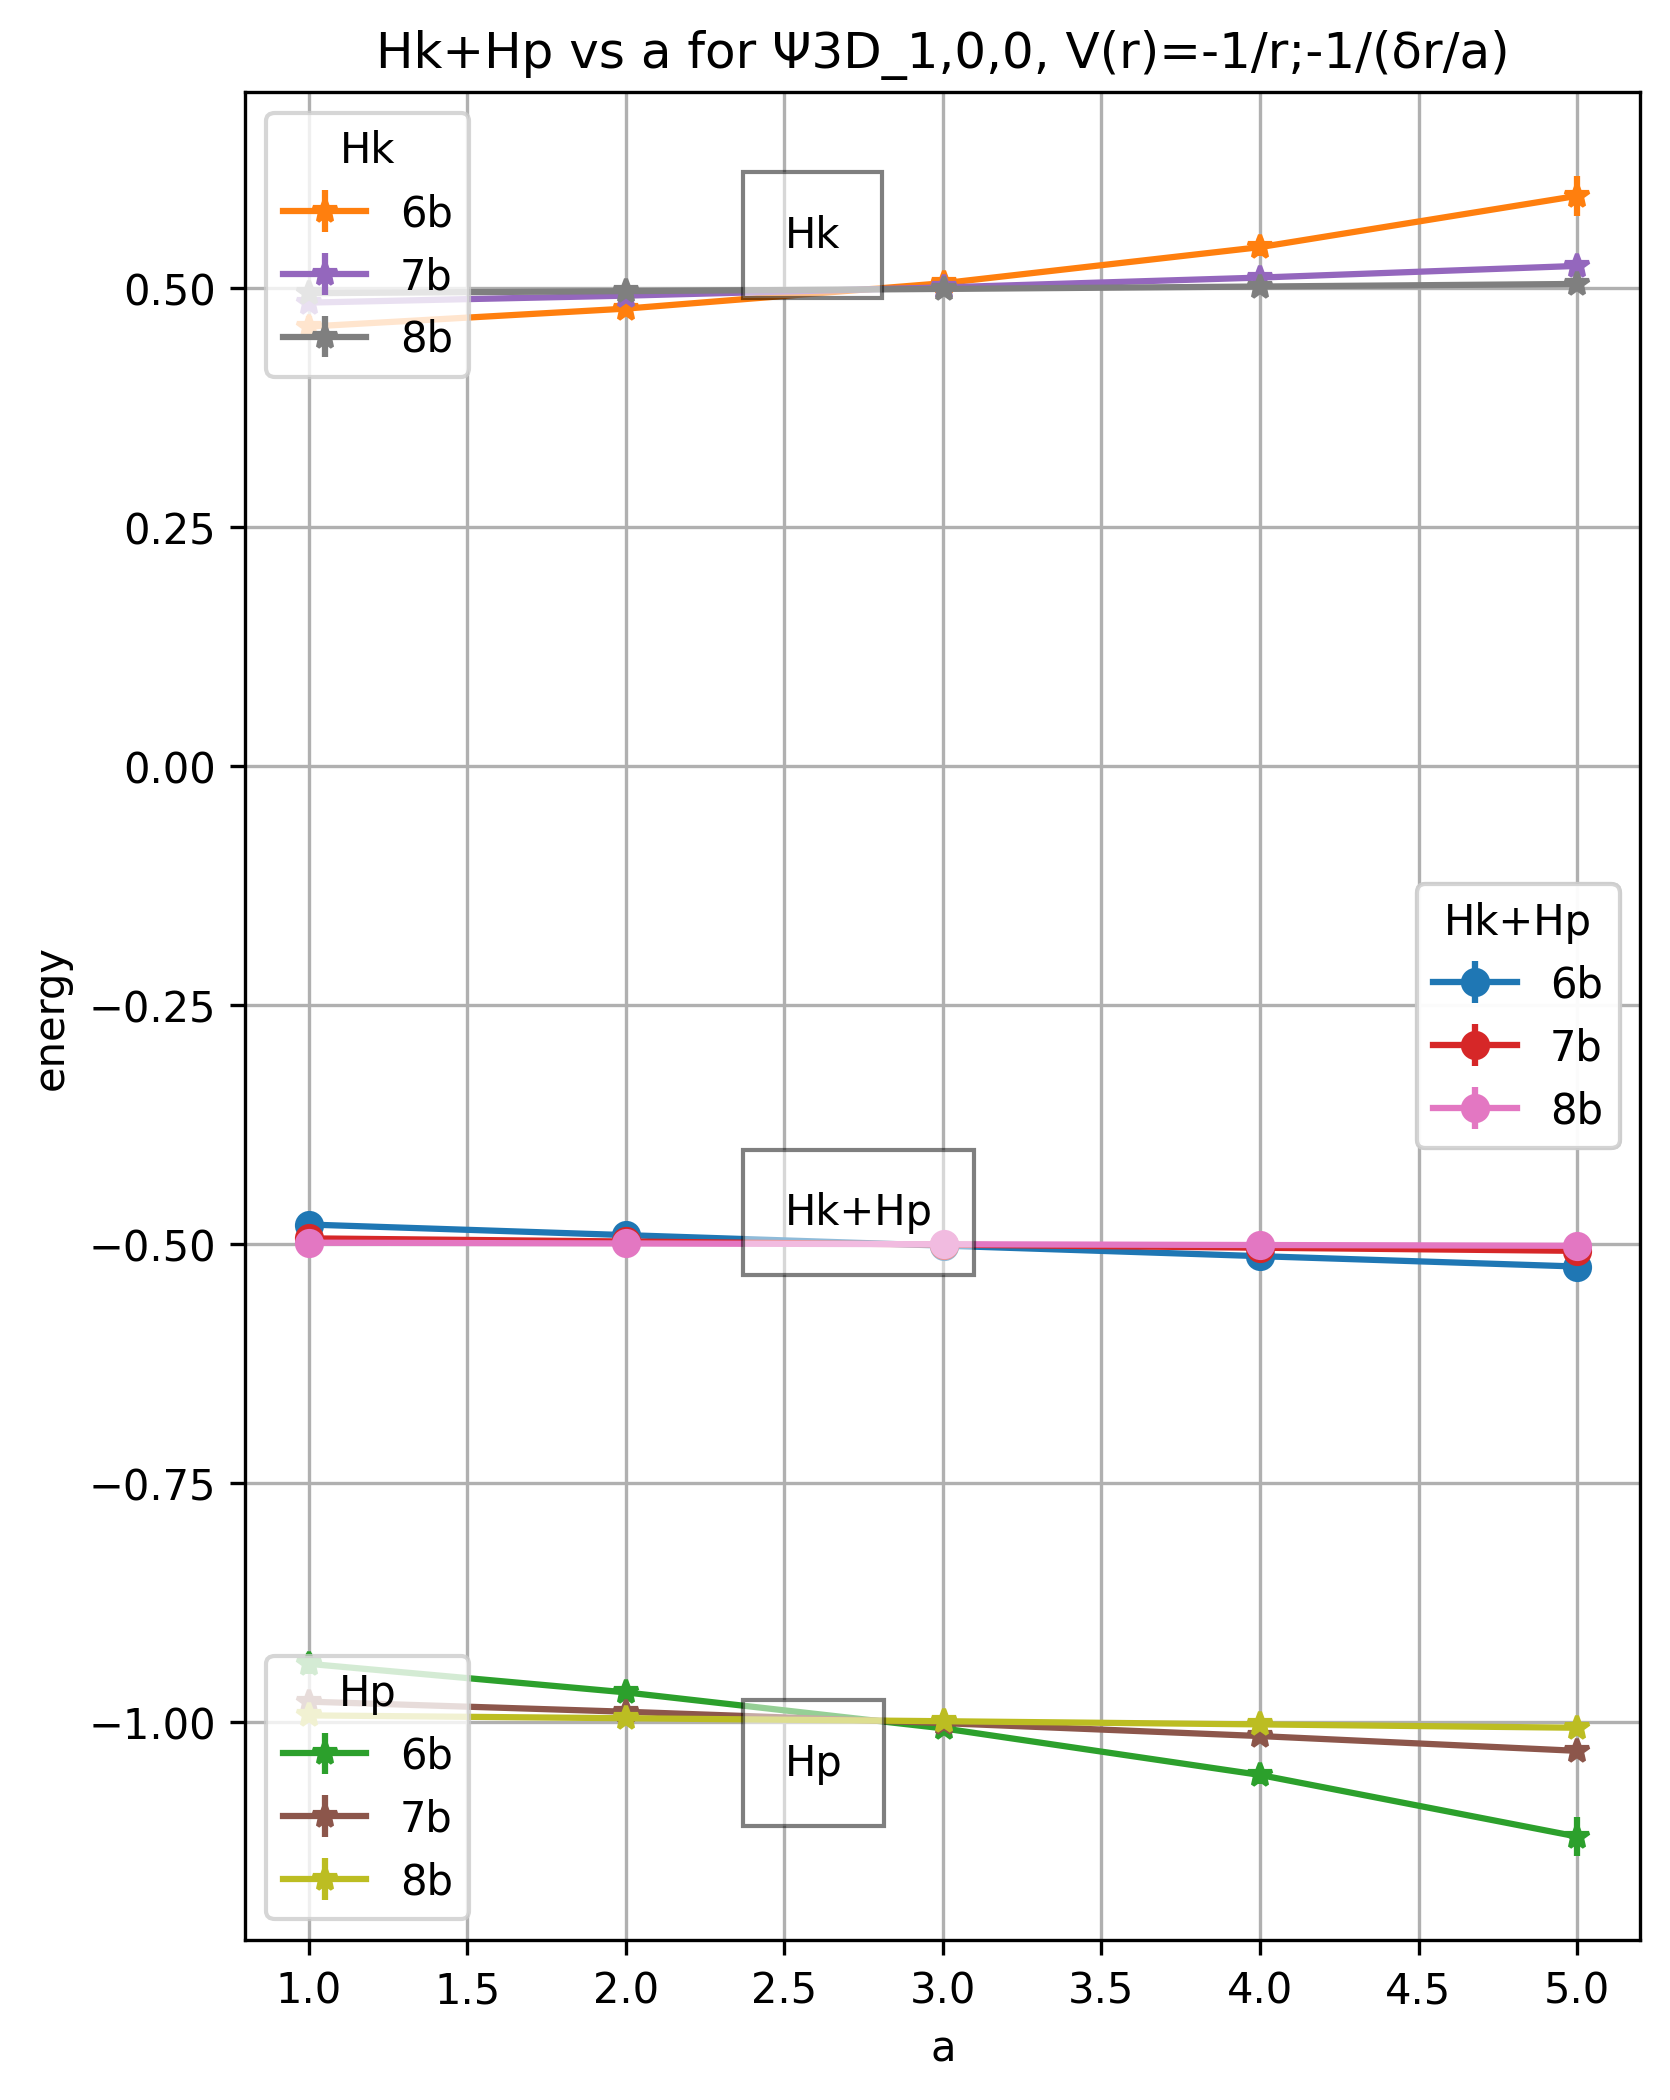
\includegraphics[width=0.6\columnwidth]{paper2025_figs/compare_energy/compare_energy_h3D_TO2_r0lim_1_0_0.png}
    \caption{3次元水素原子モデルにおいて近似式$\Hla(r)$において$\reff$の値を変えた時のエネルギー値の変化}
    \label{fig:Ha1-vs-delta1-3d}
    \begin{flushleft}\small
      
        状態$\PsiThreeD_{1,0,0}$ に対して $\reff=\deltar/a$と置き、$a$ を変化さ
        せたグラフ。全てのビット数において、$a=3$（$\reff=\deltar/3$）の時にハミ
        ルトニアンの期待値$\Hk+\Hp$ が解析解である $-0.5$ に近い値を示している。
    \end{flushleft}
\end{figure}

\end{document}
